% LaTeX source for ``Python for Informatics: Exploring Information''
% Copyright (c)  2010-  Charles R. Severance, All Rights Reserved

\chapter{Files}

\index{file}
\index{type!file}


\section{Persistence}

\index{persistence}
\index{secondary memory}

So far, we have learned how to write programs and communicate 
our intentions to the {\bf Central Processing Unit} using conditional
execution, functions, and iterations.  We have learned how to 
create and use data structures in the {\bf Main Memory}.  The CPU 
and memory are where our software works and runs.  It is where 
all of the ``thinking'' happens.  

But if you recall from our hardware architecture discussions,
once the power is turned off, anything stored in either
the CPU or main memory is erased.  So up to now, our
programs have just been transient fun exercises to learn Python.

\beforefig
\centerline{\includegraphics[height=2.50in]{figs2/arch3.eps}}
\afterfig

In this chapter, we start to work with {\bf Secondary Memory} 
(or files).
Secondary memory is not erased even when the power is turned off.  
Or in the case of a USB flash drive, the
data we write from our programs can be removed from the 
system and transported to another system.

We will primarily focus on reading and writing text files such as 
those we create in a text editor.  Later we will see how to work
with database files which are binary files, specifically designed to be read
and written through database software.

\section{Opening files}
\index{file!open}
\index{open function}
\index{function!open}

When we want to read or write a file (say on your hard drive), we first
must {\bf open} the file.  Opening the file communicates with your operating
system, which knows where the data for each file is stored.  When you open
a file, you are asking the operating system to find the file by name
and make sure the file exists.  In this example, we open the file 
{\tt mbox.txt}, which should be stored in the same folder that you
are in when you start Python.
You can download this file from 
\url{www.py4inf.com/code/mbox.txt}

\beforeverb
\begin{verbatim}
>>> fhand = open('mbox.txt')
>>> print fhand
<open file 'mbox.txt', mode 'r' at 0x1005088b0>
\end{verbatim}
\afterverb
%
\index{file handle}
If the {\tt open} is successful, the operating system returns us a 
{\bf file handle}.  The file handle is not the actual data contained
in the file, but instead it is a ``handle'' that we can use to 
read the data.   You are given a handle if the requested file
exists and you have the proper permissions to read the file.

\beforefig
\centerline{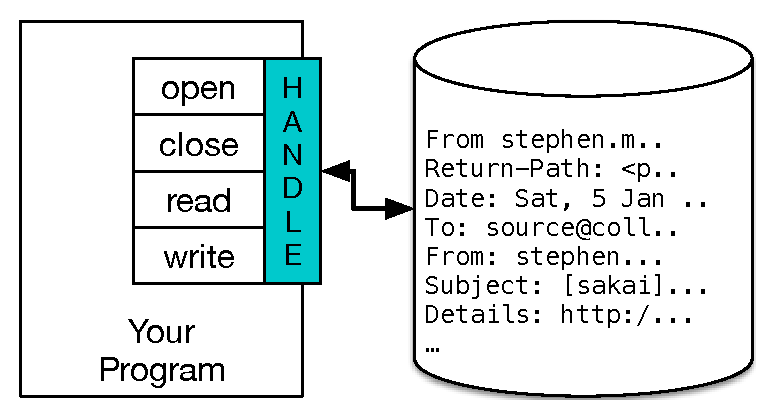
\includegraphics[height=1.75in]{figs2/handle.eps}}
\afterfig

If the file does not exist, {\tt open} will fail with a traceback and you 
will not get a handle to access the contents of the file:

\beforeverb
\begin{verbatim}
>>> fhand = open('stuff.txt')
Traceback (most recent call last):
  File "<stdin>", line 1, in <module>
IOError: [Errno 2] No such file or directory: 'stuff.txt'
\end{verbatim}
\afterverb
%
Later we will use {\tt try} and {\tt except} to deal more gracefully
with the situation where we attempt to open a file that does 
not exist.

\section{Text files and lines}

A text file can be thought of as a sequence of lines, much like a Python
string can be thought of as a sequence of characters.  For example, this
is a sample of a text file which records mail activity from various
individuals in an open source project development team:

\beforeverb
\begin{alltt}
From stephen.marquard@uct.ac.za Sat Jan  5 09:14:16 2008
Return-Path: <postmaster@collab.sakaiproject.org>
Date: Sat, 5 Jan 2008 09:12:18 -0500
To: source@collab.sakaiproject.org
From: stephen.marquard@uct.ac.za
Subject: [sakai] svn commit: r39772 - content/branches/
Details: http://source.sakaiproject.org/viewsvn/?view=rev\&rev=39772
...
\end{alltt}
\afterverb

The entire file of mail interactions is available from 
\url{www.py4inf.com/code/mbox.txt} 
and a shortened version of the file is available from
\url{www.py4inf.com/code/mbox-short.txt}.
These files are in a standard format for a file containing 
multiple mail messages. The lines which start with 
``From '' separate the messages and the lines which start 
with ``From:'' are part of the messages. 
For more information about the mbox format, see 
\url{en.wikipedia.org/wiki/Mbox}. 

To break the file into lines, there is a special character that 
represents the ``end of the line'' called the {\bf newline} character.

\index{newline}
In Python, we represent the {\bf newline} character as a backslash-n in 
string constants.  Even though this looks like two characters, it
is actually a single character.  When we look at the variable by entering
``stuff'' in the interpreter, it shows us the \verb"\n" in the string, 
but when we use {\tt print} to show the string, we see the string broken
into two lines by the newline character.

\beforeverb
\begin{verbatim}
>>> stuff = 'Hello\nWorld!'
>>> stuff
'Hello\nWorld!'
>>> print stuff
Hello
World!
>>> stuff = 'X\nY'
>>> print stuff
X
Y
>>> len(stuff)
3
\end{verbatim}
\afterverb
%

You can also see that the length of the string \verb"'X\nY'" is \emph{three}
characters because the newline character is a single character.

So when we look at the lines in a file, we need to \emph{imagine}
that there is a special invisible character called the newline at
the end of each line that marks the end of the line.  

% \beforeverb
% \begin{alltt}
% From stephen.marquard@uct.ac.za Sat Jan  5 09:14:16 2008\verb"\n"\\
% Return-Path: <postmaster@collab.sakaiproject.org>\verb"\n"\\
% Date: Sat, 5 Jan 2008 09:12:18 -0500\verb"\n"\\
% To: source@collab.sakaiproject.org\verb"\n"\\
% From: stephen.marquard@uct.ac.za\verb"\n"\\
% Subject: [sakai] svn commit: r39772 - content/branches/\verb"\n"\\
% Details: http://source.sakaiproject.org/viewsvn/?view=rev\&rev=39772\verb"\n"\\
% ...
% \end{alltt}
% \afterverb

So the newline character separates the characters 
in the file into lines.

\section{Reading files}

\index{file!reading}
\index{counter}
While the {\bf file handle} does not contain the data for the file,
it is quite easy to construct a {\tt for} loop to read through 
and count each of the lines in a file:

\beforeverb
\begin{verbatim}
fhand = open('mbox.txt')
count = 0
for line in fhand:
    count = count + 1
print 'Line Count:', count

python open.py 
Line Count: 132045
\end{verbatim}
\afterverb
%
We can use the file handle as the sequence in our {\tt for} loop.  
Our {\tt for} loop simply counts the number of lines in the 
file and prints them out.  The rough translation of the {\tt for}
loop into English is, ``for each line in the file represented by the file
handle, add one to the {\tt count} variable.''

The reason that the {\tt open} function does not read the entire file
is that the file might be quite large with many gigabytes of data.
The {\tt open} statement takes the same amount of time regardless of the
size of the file.  The {\tt for} loop actually causes the data to be 
read from the file.

When the file is read using a {\tt for} loop in this manner, Python
takes care of splitting the data in the file into separate lines using
the newline character.  Python reads each line through 
the newline and includes
the newline as the last character in the {\tt line} variable for each 
iteration of the {\tt for} loop.

Because the {\tt for} loop reads the data one line at a time, it can efficiently
read and count the lines in very large files without running 
out of main memory to store the data.  The above program can 
count the lines in any size file using very little memory since 
each line is read, counted, and then discarded.

If you know the file is relatively small compared to the size of 
your main memory, you can read the whole file into one string
using the {\tt read} method on the file handle.

\beforeverb
\begin{verbatim}
>>> fhand = open('mbox-short.txt')
>>> inp = fhand.read()
>>> print len(inp)
94626
>>> print inp[:20]
From stephen.marquar
\end{verbatim}
\afterverb
%
In this example, the entire contents (all 94,626 characters) 
of the file {\tt mbox-short.txt} are read directly into the 
variable {\tt inp}.  We use string slicing to print out the first
20 characters of the string data stored in {\tt inp}.

When the file is read in this manner, all the characters including 
all of the lines and newline characters are one big string 
in the variable {\bf inp}.  
Remember that this form of the {\tt open} function should only be used
if the file data will fit comfortably in the main memory 
of your computer.

If the file is too large to fit in main memory, you should write
your program to read the file in chunks using a {\tt for} or {\tt while}
loop.

\section{Searching through a file}

When you are searching through data in a file, it
is a very common pattern to read through a file, ignoring most
of the lines and only processing lines which meet a particular condition.
We can combine the pattern for reading a file with string methods
to build simple search mechanisms.

\index{filter pattern}
\index{pattern!filter}
For example, if we wanted to read a file and only print out lines
which started with the prefix ``From:'', we could use the 
string method {\bf startswith} to select only those lines with
the desired prefix:

\beforeverb
\begin{verbatim}
fhand = open('mbox-short.txt')
for line in fhand:
    if line.startswith('From:') :
        print line
\end{verbatim}
\afterverb
%
When this program runs, we get the following output:

\beforeverb
\begin{verbatim}
From: stephen.marquard@uct.ac.za

From: louis@media.berkeley.edu

From: zqian@umich.edu

From: rjlowe@iupui.edu
...
\end{verbatim}
\afterverb
%
The output looks great since the only lines we are seeing are those 
which start with ``From:'', but why are we seeing the extra blank
lines?  This is due to that invisible {\bf newline} character.
Each of the lines ends with a newline, so the {\tt print} 
statement prints the string in the variable {\bf line} which includes
a newline and then {\tt print} adds \emph{another} newline, resulting
in the double spacing effect we see.

We could use line slicing to print all but the last character, but 
a simpler approach is to use the {\bf rstrip} method which strips
whitespace from the right side of a string as follows:

\beforeverb
\begin{verbatim}
fhand = open('mbox-short.txt')
for line in fhand:
    line = line.rstrip()
    if line.startswith('From:') :
        print line
\end{verbatim}
\afterverb
%
When this program runs, we get the following output:

\beforeverb
\begin{verbatim}
From: stephen.marquard@uct.ac.za
From: louis@media.berkeley.edu
From: zqian@umich.edu
From: rjlowe@iupui.edu
From: zqian@umich.edu
From: rjlowe@iupui.edu
From: cwen@iupui.edu
...
\end{verbatim}
\afterverb
%
As your file processing programs get more complicated, you may want 
to structure your search loops using {\tt continue}.  The basic idea 
of the search loop is that you are looking for ``interesting'' lines
and effectively skipping ``uninteresting'' lines.  And then when we
find an interesting line, we do something with that line.

We can structure the loop to follow the
pattern of skipping uninteresting lines as follows:

\beforeverb
\begin{verbatim}
fhand = open('mbox-short.txt')
for line in fhand:
    line = line.rstrip()
    # Skip 'uninteresting lines'
    if not line.startswith('From:') :
        continue
    # Process our 'interesting' line
    print line
\end{verbatim}
\afterverb
%
The output of the program is the same.  In English, the 
uninteresting lines are those which do not start 
with ``From:'', which we skip using {\tt continue}.
For the ``interesting'' lines (i.e., those that start with ``From:'')
we perform the processing on those lines.

We can use the {\tt find} string method to simulate a text editor
search that finds lines where the search string is anywhere in the line.  
Since {\tt find} looks for an occurrence of a string within another
string and either returns the position of the string or -1 if the string
was not found, we can write the following loop to show lines which
contain the string ``@uct.ac.za'' (i.e., they come from the University 
of Cape Town in South Africa):

\beforeverb
\begin{verbatim}
fhand = open('mbox-short.txt')
for line in fhand:
    line = line.rstrip()
    if line.find('@uct.ac.za') == -1 : 
        continue
    print line
\end{verbatim}
\afterverb
%
Which produces the following output:

\beforeverb
\begin{verbatim}
From stephen.marquard@uct.ac.za Sat Jan  5 09:14:16 2008
X-Authentication-Warning: set sender to stephen.marquard@uct.ac.za using -f
From: stephen.marquard@uct.ac.za
Author: stephen.marquard@uct.ac.za
From david.horwitz@uct.ac.za Fri Jan  4 07:02:32 2008
X-Authentication-Warning: set sender to david.horwitz@uct.ac.za using -f
From: david.horwitz@uct.ac.za
Author: david.horwitz@uct.ac.za
...
\end{verbatim}
\afterverb
%

\section{Letting the user choose the file name}

We really do not want to have to edit our Python code
every time we want to process a different file.  It would 
be more usable to ask the user to enter the file name string 
each time the program runs so they can use our 
program on different files without changing the Python code.

This is quite simple to do by reading the file name from
the user using \verb"raw_input" as follows:

\beforeverb
\begin{verbatim}
fname = raw_input('Enter the file name: ')
fhand = open(fname)
count = 0
for line in fhand:
    if line.startswith('Subject:') :
        count = count + 1
print 'There were', count, 'subject lines in', fname
\end{verbatim}
\afterverb
%
We read the file name from the user and place it in a variable
named {\tt fname} and open that file.  Now we can run the program 
repeatedly on different files.

\beforeverb
\begin{verbatim}
python search6.py 
Enter the file name: mbox.txt
There were 1797 subject lines in mbox.txt

python search6.py 
Enter the file name: mbox-short.txt
There were 27 subject lines in mbox-short.txt
\end{verbatim}
\afterverb
%
Before peeking at the next section, take a look at the above program
and ask yourself, ``What could go possibly wrong here?'' or ``What might our
friendly user do that would cause our nice little program to 
ungracefully exit with a traceback, making us look not-so-cool 
in the eyes of our users?''

\section{Using {\tt try, except,} and {\tt open}}

I told you not to peek.  This is your last chance.

What if our user types something that is not a file name?

\beforeverb
\begin{verbatim}
python search6.py 
Enter the file name: missing.txt
Traceback (most recent call last):
  File "search6.py", line 2, in <module>
    fhand = open(fname)
IOError: [Errno 2] No such file or directory: 'missing.txt'

python search6.py 
Enter the file name: na na boo boo
Traceback (most recent call last):
  File "search6.py", line 2, in <module>
    fhand = open(fname)
IOError: [Errno 2] No such file or directory: 'na na boo boo'
\end{verbatim}
\afterverb
%
Do not laugh, users will eventually do every possible thing they can do 
to break your programs---either on purpose or with malicious intent.
As a matter of fact, an important part of any software development
team is a person or group called {\bf Quality Assurance} (or QA for short)
whose very job it is to do the craziest things possible in an attempt
to break the software that the programmer has created.

\index{Quality Assurance}
\index{QA}
The QA team is responsible for finding the flaws in programs before 
we have delivered the program to the end users who may be purchasing the
software or paying our salary to write the software.  So the QA team
is the programmer's best friend.

\index{try statement}
\index{statement!try}
\index{open function}
\index{function!open}
\index{exception!IOError}
\index{IOError}
So now that we see the flaw in the program, we can elegantly fix it using
the {\tt try}/{\tt except} structure.  We need to assume that the {\tt open}
call might fail and add recovery code when the {\tt open} fails
as follows:

\beforeverb
\begin{verbatim}
fname = raw_input('Enter the file name: ')
try:
    fhand = open(fname)
except:
    print 'File cannot be opened:', fname
    exit()

count = 0
for line in fhand:
    if line.startswith('Subject:') : 
        count = count + 1
print 'There were', count, 'subject lines in', fname
\end{verbatim}
\afterverb
%
The {\tt exit} function terminates the program.  It is a function
that we call that never returns.  Now when our user (or 
QA team) types in silliness or bad file names, 
we ``catch'' them and recover gracefully:

\beforeverb
\begin{verbatim}
python search7.py
Enter the file name: mbox.txt
There were 1797 subject lines in mbox.txt

python search7.py
Enter the file name: na na boo boo
File cannot be opened: na na boo boo
\end{verbatim}
\afterverb
%
\index{Pythonic}
Protecting the {\tt open} call is a good example 
of the proper use of {\tt try}
and {\tt except} in a Python program.  We use the term
``Pythonic'' when we are doing something the ``Python
way''.  We might say that the above example is 
the Pythonic way to open a file.

Once you become more skilled in Python, you can engage
in repartee with other Python programmers to decide
which of two equivalent solutions to a problem is 
``more Pythonic''.  The goal to be ``more Pythonic'' 
captures the notion that programming is part engineering
and part art.  We are not always interested
in just making something work, we also want
our solution to be elegant and to be appreciated as 
elegant by our peers.


\section{Writing files}

\index{file!writing}

To write a file, you have to open it with mode
\verb"'w'" as a second parameter:

\beforeverb
\begin{verbatim}
>>> fout = open('output.txt', 'w')
>>> print fout
<open file 'output.txt', mode 'w' at 0xb7eb2410>
\end{verbatim}
\afterverb
%
If the file already exists, opening it in write mode clears out
the old data and starts fresh, so be careful!
If the file doesn't exist, a new one is created.

The {\tt write} method of the file handle object 
puts data into the file.

\beforeverb
\begin{verbatim}
>>> line1 = "This here's the wattle,\n"
>>> fout.write(line1)
\end{verbatim}
\afterverb
%
\index{newline}
Again, the file object keeps track of where it is, so if
you call {\tt write} again, it adds the new data to the end.

We must make sure to manage the ends of lines as we write
to the file by explicitly inserting the newline character
when we want to end a line.  The {\tt print} statement 
automatically appends a newline, but the {\tt write} 
method does not add the newline automatically.

\beforeverb
\begin{verbatim}
>>> line2 = 'the emblem of our land.\n'
>>> fout.write(line2)
\end{verbatim}
\afterverb
%
When you are done writing, you have to close the file
to make sure that the last bit of data is physically written
to the disk so it will not be lost if the power goes off.

\beforeverb
\begin{verbatim}
>>> fout.close()
\end{verbatim}
\afterverb
%
We could close the files which we open for read as well, 
but we can be a little sloppy if we are only opening a few
files since Python makes sure that all open files are 
closed when the program ends.  When we are writing files, 
we want to explicitly close the files so as to leave nothing
to chance.

\index{close method}
\index{method!close}


\section{Debugging}

\index{debugging}
\index{whitespace}

When you are reading and writing files, you might run into problems
with whitespace.  These errors can be hard to debug because spaces,
tabs, and newlines are normally invisible:

\beforeverb
\begin{verbatim}
>>> s = '1 2\t 3\n 4'
>>> print s
1 2	 3
 4
\end{verbatim}
\afterverb

\index{repr function}
\index{function!repr}
\index{string representation}

The built-in function {\tt repr} can help.  It takes any object as an
argument and returns a string representation of the object.  For
strings, it represents whitespace
characters with backslash sequences:

\beforeverb
\begin{verbatim}
>>> print repr(s)
'1 2\t 3\n 4'
\end{verbatim}
\afterverb

This can be helpful for debugging.

One other problem you might run into is that different systems
use different characters to indicate the end of a line.  Some
systems use a newline, represented \verb"\n".  Others use
a return character, represented \verb"\r".  Some use both.
If you move files between different systems, these inconsistencies
might cause problems.

\index{end of line character}

For most systems, there are applications to convert from one
format to another.  You can find them (and read more about this
issue) at \url{wikipedia.org/wiki/Newline}.  Or, of course, you
could write one yourself.

% TBD - Doesn't Python take care of this for us????

\section{Glossary}

\begin{description}

\item[catch:] To prevent an exception from terminating
a program using the {\tt try} and {\tt except} statements.
\index{catch}

\item[newline:] A special character used in files and strings to indicate
the end of a line.
\index{newline}

\item[Pythonic:] A technique that works elegantly in Python.
``Using try and except is the \emph{Pythonic} way to recover from 
missing files''.
\index{Pythonic}

\item[Quality Assurance:] A person or team focused on insuring the 
overall quality of a software product.  QA is often involved 
in testing a product and identifying problems before the product 
is released.
\index{Quality Assurance}
\index{QA}

\item[text file:] A sequence of characters stored in permanent
storage like a hard drive.
\index{text file}

\end{description}


\section{Exercises}

\begin{ex}
Write a program to read through a file and print the contents 
of the file (line by line) all in upper case.  Executing the program 
will look as follows:

\beforeverb
\begin{verbatim}
python shout.py
Enter a file name: mbox-short.txt
FROM STEPHEN.MARQUARD@UCT.AC.ZA SAT JAN  5 09:14:16 2008
RETURN-PATH: <POSTMASTER@COLLAB.SAKAIPROJECT.ORG>
RECEIVED: FROM MURDER (MAIL.UMICH.EDU [141.211.14.90])
	 BY FRANKENSTEIN.MAIL.UMICH.EDU (CYRUS V2.3.8) WITH LMTPA;
	 SAT, 05 JAN 2008 09:14:16 -0500
\end{verbatim}
\afterverb
%
You can download the file from
\url{www.py4inf.com/code/mbox-short.txt}
\end{ex}

\begin{ex}
Write a program 
to prompt for a file name, and then read through the file 
and look for lines of the form:

\beforeverb
\begin{alltt}
X-DSPAM-Confidence: {\bf 0.8475}
\end{alltt}
\afterverb

When you encounter a line that starts with 
``X-DSPAM-Confidence:'' pull apart the line to extract the
floating-point number on the line.  Count these lines and
then compute the total of the spam confidence values from
these lines. When you reach the end of the file, print out
the average spam confidence.

\beforeverb
\begin{verbatim}
Enter the file name: mbox.txt
Average spam confidence: 0.894128046745

Enter the file name: mbox-short.txt
Average spam confidence: 0.750718518519
\end{verbatim}
\afterverb
%
Test your file on the {\tt mbox.txt} and {\tt mbox-short.txt} files.
\end{ex}


\begin{ex}
Sometimes when programmers get bored or want to have a bit of fun,
they add a harmless {\bf Easter Egg} to their program 
(\url{en.wikipedia.org/wiki/Easter_egg_(media)}). Modify the program
that prompts the user for the file name so that it prints a funny
message when the user types in the exact file name ``na na boo boo''. 
The program should behave normally for all other files which exist
and don't exist.  Here is a sample execution of the program:

\beforeverb
\begin{verbatim}
python egg.py 
Enter the file name: mbox.txt
There were 1797 subject lines in mbox.txt

python egg.py 
Enter the file name: missing.tyxt
File cannot be opened: missing.tyxt

python egg.py 
Enter the file name: na na boo boo
NA NA BOO BOO TO YOU - You have been punk'd!
\end{verbatim}
\afterverb
%
We are not encouraging you to put Easter Eggs in your 
programs---this is just an exercise.

\end{ex}

